\documentclass[12pt,a4paper,openright,twoside]{book}
\usepackage[utf8]{inputenc}
\usepackage{disi-thesis}
\usepackage{code-lstlistings}
\usepackage{notes}
\usepackage{shortcuts}
\usepackage{acronym}

\school{\unibo}
\programme{Corso di Laurea Magistrale in Ingegneria e Scienze Informatiche}
\title{MYOP - Make your own poll \\
Libreria multipiattaforma \\
a supporto della \\
democrazia digitale
}
\author{Jacopo Corina}
\date{\today}
\subject{Laboratorio di sistemi software}
\supervisor{Prof. Danilo Pianini}
\session{III}
\academicyear{2022-2023}

% Definition of acronyms
\acrodef{IoT}{Internet of Thing}
\acrodef{vm}[VM]{Virtual Machine}


\mainlinespacing{1.5} % line spacing in mainmatter, comment to default (1)

\begin{document}

\frontmatter 
\frontispiece

\begin{abstract}	
Max 2000 characters, strict.
\end{abstract}

\begin{dedication} % this is optional
Ai miei genitori
\end{dedication}

\begin{acknowledgements} % this is optional
Optional. Max 1 page.
\end{acknowledgements}

%----------------------------------------------------------------------------------------
\tableofcontents   
\listoffigures     % (optional) comment if empty
\lstlistoflistings % (optional) comment if empty
%----------------------------------------------------------------------------------------

\mainmatter

%----------------------------------------------------------------------------------------
\chapter{Introduzione}
\label{chap:introduction}
%----------------------------------------------------------------------------------------
\chapter{Democrazia digitale}
Il termine \textit{Democrazia}, derivante dal greco \textit{governo del popolo},
indica un forma di governo il quale, attraverso una forma diretta che coinvolge attivamente
la popolazione nelle decisioni o attraverso forme rappresentative che coinvolgono figure intermediarie,
pone in ogni caso il potere sul popolo stesso.

Nelle epoche successive alle prime forme di democrazia "unanime", complice anche la complessità
delle materie da amministrare e il numero dei partecipanti fisici, la democrazia
indiretta ha preso la maggior diffusione. 

La recente modernizzazione tecnologica ha aperto un ventaglio di possibilità tali da
permettere un ritorno ad un controllo più diretto da parte della collettività.
La \textit{democrazia digitale} (o \textit{e-democracy}) è la pratica della democrazia attraverso 
l’utilizzo di strumenti digitali e tecnologie, avente l’obiettivo di intensificare la partecipazione 
attiva del membro della comunità.
Queste tecnologie permettono di facilitare l'esercizio di ulteriori forme di democrazie,
come quella partecipata, in cui i cittadini, piuttosto che
sostituirsi ai rappresentanti, forniscono idee sullo sviluppo dell'indirizzo di governo
permettendo così di creare un collettore di confronto ed analisi di situazioni differenti.

Tuttavia, è necessario considerare che un uso eccessivamente estensivo di questi strumenti
può portare al rischi di coinvolgere persone che non hanno abbastanza competenze relativamente 
a temi delicati, ad esempio le politiche sociali. 

Inoltre, nonostante la virtualizzazione della partecipazione permette alle fasce più disagiate di essere
maggiormente coinvolte, introduce un motivo di scetticismo relativamente alla componente tecnologica
in ambito di sicurezza informatica, segretezza e manipolazione del voto.

L'applicazione più comune di queste tecnologie emergenti è legata al mondo della politica:
sono degni di nota casi come l'Estonia, che dal 2005 rende possibili via Internet le votazioni
per elezioni e referendum, e l'Islanda che tramite un ambizioso progetto tenta di riscrivere 
la costituzione con l'apporto dei cittadini. In Italia possiamo rilevare l'applicativo PartecipaMi,
organizzata per mettere in contatto la popolazione milanese con l'amministrazione comunale.

Inoltre, queste soluzioni sono spesso adottate da partiti o movimenti politici per avviare iniziative
e votazioni interne tra i membri, come nel caso del Partito Pirata tedesco in Germania (piattaforma LiquidFeedback),
o il Movimento 5 Stelle in Italia (piattaforma Rousseau).
Sistemi come LiquidFeedback, OpenDCN, Airesis, essendo strutturati come applicativi end-to-end,
pongo molta enfasi sull'interazione tra utenti, la presentazione e validazione di proposte,
l'eventuale presenza di deleghe, l'espressione del voto tramite una lista di preferenze, ma
non permettono la variazione delle logiche di selezione del vincitore da applicare\cite{Trapanese:2018}.

In altri casi, una fase di analisi iniziale poco trasversale, ha portato a dar maggior risalto
ad aspetti non funzionali, come la privacy, rispetto a quelli funzionali come il modello di democrazia
da applicare, che per alcuni aspetti rimane implicito. 
La mancanza di elementi formalizzanti, che descrivono dettagliatamente tutti gli step applicati nel
processo, e le variazioni ed evoluzioni che vengono apportate nel tempo, portano alla divergenza di flusso rispetto all'idea iniziale, 
e di conseguenza confondere gli utilizzatori e scoraggiare l'utilizzo della piattaforma\cite{Pianini:2019}.

%modello implicito, sforzi iniziali ma analisi poco dettagliata lascia punti scoperti, si da maggior risalito a req non funzionali che funzionali
%aumentare curva apprendimento e incertezza aumenta con il numero di funzionalità e impatto negativo sull' usabilità

%----------------------------------------------------------------------------------------
\chapter{Automazione e versionamento artefatti}

\section{Kotlin Multiplatform}
Spiegare brevemente in cosa consiste, con immagini a supporto

\section{Github}

    \subsection{Github Actions}
    Spiegazione funzionamento pipelines

    \subsection{Github Pages}
    Hosting di documentazione

    \subsection{Artefatti}
    Nota per il Prof.
    Non so se va spiegata qui la pubblicazione su Maven central/ github packages / npm
    oppure se parlarne direttamente nell' implementazione
%----------------------------------------------------------------------------------------
\chapter{Analisi}
In questa parte metterei dettagli su votazioni a singola preferenza 
e votazioni a lista di preferenze (es.Condorcet)
\section{Requisiti}

    \subsection{Requisiti funzionali}

    \subsection{Requisiti non funzionali}

\section{Modello del dominio}
%----------------------------------------------------------------------------------------
\chapter{Design}
%----------------------------------------------------------------------------------------
\chapter{Implementazione}

\section{DSL }

\section{Librerie multiplatform utilizzate}

\section{Pubblicazione di artefatti}
Spiegare brevemente i passaggi necessari che sono stati fatti per arrivare
alle pubblicazioni

\section{Pubblicazione della documentazione}
spiegare la creazione di un nuovo workflow, e collegato a quelli esistenti
%----------------------------------------------------------------------------------------
\chapter{Valutazione}

\section{Test realizzati}
Descrivere le varie situazioni che sono andato a controllare,
mettendo dettagli solo per i casi più complicati

\section{Sperimentazione con Ergast API}
Estratti di demo che ho realizzato usando i dati della Formula 1
%----------------------------------------------------------------------------------------
\chapter{Conclusioni}




%Write your intro here.
%\sidenote{Add sidenotes in this way. They are named after the author of the thesis}

%You can use acronyms that your defined previously,
%You can use acronyms that your defined previously,
%such as \ac{IoT}.
%
%If you use acronyms twice,
%they will be written in full only once
%(indeed, you can mention the \ac{IoT} now without it being fully explained).
%
%In some cases, you may need a plural form of the acronym.
%
%For instance,
%that you are discussing \acp{vm},
%you may need both \ac{vm} and \acp{vm}.

%\paragraph{Structure of the Thesis}

%\note{At the end, describe the structure of the paper}

%\chapter{State of the art}

%I suggest referencing stuff as follows: \cref{fig:random-image} or \Cref{fig:random-image}

%\begin{figure}
%    \centering
%    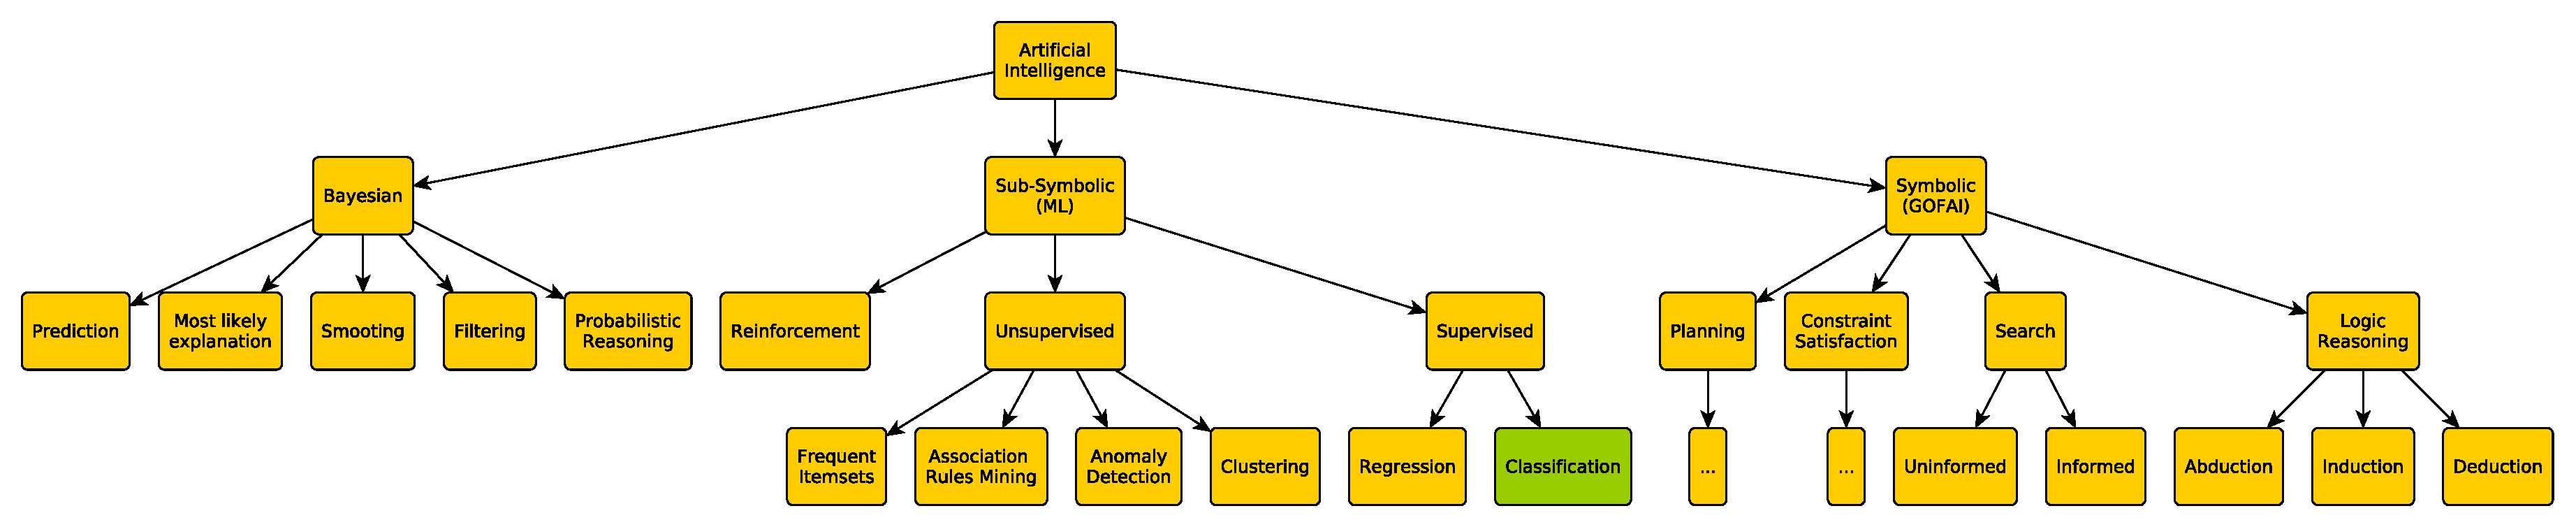
\includegraphics[width=.8\linewidth]{figures/random-image.pdf}
%    \caption{Some random image}
%    \label{fig:random-image}
%\end{figure}

%\section{Some cool topic}

%\chapter{Contribution}

%You may also put some code snippet (which is NOT float by default), eg: \cref{lst:random-code}.

%\lstinputlisting[float,language=Java,label={lst:random-code}]{listings/HelloWorld.java}

%\section{Fancy formulas here}

%----------------------------------------------------------------------------------------
% BIBLIOGRAPHY
%----------------------------------------------------------------------------------------

\backmatter

\nocite{*} % comment this to only show the referenced entries from the .bib file


\bibliographystyle{alpha}
\bibliography{bibliography}

\end{document}